\documentclass[sigconf]{acmart}
% \usepackage[hyphens]{url}
% \usepackage[usenames,dvipsnames]{color}
\usepackage{comment}
\usepackage{float}
\usepackage{lipsum}
\usepackage{pifont} %used for tickmark and crosses.
% \usepackage[english]{babel}
% \usepackage{array}
\usepackage{multirow}
% \usepackage{amssymb}
% \usepackage{amsthm}
\usepackage{amsmath}
\usepackage[normalem]{ulem}
\usepackage{xspace}
\usepackage{datetime}

% To support subfigures
%\usepackage{caption}
%\usepackage{subcaption}

% \usepackage{graphicx}

%%%%%%%%%% verbatim related
\usepackage{fancyvrb}
\fvset{framesep=2mm,fontsize=\scriptsize,framerule=.1mm,numbersep=1mm,commandchars=\\\{\}}
\usepackage{listings}

%%%%%%%%%%%%%%%%%%%% pseudocode-related stuff
%\usepackage[usenames,dvipsnames]{xcolor}
\newcommand{\codecomment}[1]{\textcolor[rgb]{0.133,0.445,0.133}{#1}}
\usepackage{algorithm}
\usepackage[noend]{algpseudocode}
% \usepackage{algorithmic}
\newfloat{algorithm}{t}{lop}
% change indentation!!
%\setlength\fboxsep{0pt}
\renewcommand\algorithmicindent{1em}
%\newcommand{\INDSTATE}[1][1]{\State\hspace{#1\algorithmicindent}}
% \newcommand{\INDSTATE}[1][1]{\State\hspace{2em}}
%%%%%%%%%%%%%%%%%%%%

% float control
\renewcommand{\topfraction}{0.9}

\widowpenalty=10000
\clubpenalty=10000

% \usepackage[small,compact]{titlesec}

% \usepackage{savetrees}

%%%%%%%%%%%%%%%%%%%%

\newtheorem{mydef}{Definition}
\newtheorem{theorem}{Theorem}[section]
\newsavebox{\verbbox}
% \usepackage[stable]{footmisc}

\newif\ifrev

%%%%%%%%%%%%%%%%%%
\usepackage{hyperref}

\newcommand{\PPH}{{\sc \{Pass\}}\xspace}
\hypersetup{%
  pdftitle = {Put your title here.  It will show up when printing or looking at PDF details},
  pdfkeywords = {},
 % pdfauthor = { Justin Cappos},
  pdfauthor = { Names removed for anonymous submission},
  bookmarksnumbered,
  bookmarksopen=true,
  colorlinks=true,
  urlcolor=[rgb]{.35,0,0},
  linkcolor=[rgb]{.35,0,0},
  citecolor=[rgb]{.35,0,0},
  pdfstartview={FitH},
}


%%%%%%%%%%%%%%%%%%
% COMMENT OUT NEXT LINE TO HIDE TODOs
\revtrue
%%%%%%%%%%%%%%%%%%

\ifrev
  \newcommand{\todo}[1]{{\color{red} [TODO: #1]}}
\else
  \newcommand{\todo}[1]{}
\fi

\newcommand{\tickmark}{\ding{51}}
\newcommand{\xmark}{\ding{55}}

\newcommand*\samethanks[1][\value{footnote}]{\footnotemark[#1]}

\usepackage{ifthen}
\usepackage[normalem]{ulem} % for \sout
\usepackage{xcolor}
\let\lneq\undefined  % removes amssymb conflict with some packages
%\usepackage{amssymb}
\newcommand{\ra}{$\rightarrow$}
\newboolean{showedits}
\setboolean{showedits}{true} % toggle to show or hide edits
\ifthenelse{\boolean{showedits}}
{
	\newcommand{\ugh}[1]{\textcolor{red}{\uwave{#1}}} % please rephrase
	\newcommand{\ins}[1]{\textcolor{blue}{\uline{#1}}} % please insert
	\newcommand{\del}[1]{\textcolor{red}{\sout{#1}}} % please delete
	\newcommand{\chg}[2]{\textcolor{red}{\sout{#1}}{\ra}\textcolor{blue}{\uline{#2}}} % please change
}{
	\newcommand{\ugh}[1]{#1} % please rephrase
	\newcommand{\ins}[1]{#1} % please insert
	\newcommand{\del}[1]{} % please delete
	\newcommand{\chg}[2]{#2}
}

\newboolean{showcomments}
%\setboolean{showcomments}{true}
\setboolean{showcomments}{true}
\newcommand{\id}[1]{$-$Id: scgPaper.tex 32478 2010-04-29 09:11:32Z oscar $-$}
\newcommand{\yellowbox}[1]{\fcolorbox{gray}{yellow}{\bfseries\sffamily\scriptsize#1}}
\newcommand{\triangles}[1]{{\sf\small$\blacktriangleright$\textit{#1}$\blacktriangleleft$}}
\ifthenelse{\boolean{showcomments}}
%{\newcommand{\nb}[2]{{\yellowbox{#1}\triangles{#2}}}
{\newcommand{\nbc}[3]{
 {\colorbox{#3}{\bfseries\sffamily\scriptsize\textcolor{white}{#1}}}
 {\textcolor{#3}{\sf\small$\blacktriangleright$\textit{#2}$\blacktriangleleft$}}}
 \newcommand{\version}{\emph{\scriptsize\id}}}
{\newcommand{\nbc}[3]{}
 \renewcommand{\ugh}[1]{#1} % please rephrase
 \renewcommand{\ins}[1]{#1} % please insert
 \renewcommand{\del}[1]{} % please delete
 \renewcommand{\chg}[2]{#2} % please change
 \newcommand{\version}{}}
\newcommand{\nb}[2]{\nbc{#1}{#2}{orange}}

\definecolor{jccolor}{rgb}{0.2,0.4,0.6}
\definecolor{clcolour}{rgb}{0.5,0.7,0.9}
\newcommand\cappos[1]{\nbc{JC}{#1}{jccolor}}
\usepackage{wasysym}


\begin{document}

\title{Cybersecurity Shuffle: Comprehension is in the Cards}


% enable this to de-anonymize!
%\newcommand{\showurlx}{{\url{https://whatever_the_url.is}}}
\newcommand{\showurlx}{[redacted]}

\author{
%\IEEEauthorblockN{Justin Cappos}\\
%New York University\\
%jcappos@nyu.edu
%\and
Use whatever template the conference provides for the paper.tex file.
% copy the following lines to add more authors
% \and
% {\rm Name}\\
%Name Institution
}

\begin{abstract}

One of the main challenges
in designing lessons
for an introductory
information security class
is how to present new technical concepts
in a manner comprehensible to students
with widely different backgrounds. A non-traditional approach
can help students engage with the material
and master these unfamiliar ideas.
We have devised a series of lessons that teach important information security
topics, such as social engineering,
side-channel attacks,
and
attacks on randomness
using card magic.
Each lesson
centers around a card trick
that allows the instructor
to simulate the described attack
in a way that makes sense even for those who have no prior technical
background.
In this paper,
we describe our experience using these lessons in teaching
cybersecurity topics
to high school students with limited computer science education.
Students were assessed
before and after the demonstration
to gauge their mastery of the material,
and their
opinions on each lesson.
Our results indicate that students enjoyed the lesson
and their pre- and post-test scores improved by between 15\% and 30\%.


\end{abstract}

%Hand-waving away the technical background behind these concepts is bad...
%
%...and undermines student's motivation to learn and understand the material.
%
%Bypassing the need for technical explanation while preserving the main
%  focus of the lesson.


\maketitle

\section{Introduction}
\label{SEC:introduction}

When teaching technical topics
in introductory courses,
it can be challenging
to present information
in a way that is approachable
for students of varying
experience levels
or educational backgrounds.
This is particularly true
for information security classes
where an adversarial mindset
is required
to fully appreciate the impact of attacks and the effort required to
defend against them.
Thinking in this way
may not come naturally
to many students,
as evidenced
by the continuing success of phishing attacks
and scams in the real world.
What is needed
is a way
to relate information security concepts
to novice students
in a manner
that is engaging enough
to build an appreciation for the material,
and relatable enough that the students do not feel lost.

In this paper
we develop three card-magic-based lessons
for introductory information security courses
that take inspiration
from the success others have had
in using magic
to explain computer science concepts.
The key to teaching these unknown concepts
lies in a common pedagogical technique
known as scaffolding.
Scaffolding is a process that lets students build
new knowledge on existing knowledge.
As explained in one source,
``students are escorted and monitored through learning
activities that function as interactive conduits to get
them to the next stage~\cite{raymond2000}.''
In the field of computer science,
several researchers have reported success in using card
tricks—something most people
have seen either at a birthday party
or on television— to teach complex concepts.
We decided to employ this technique to teach how three types
of attacks -- social engineering, side channel attacks, and attacks on
randomness -- work in the real world.
The specific trick and presentation technique
for each lesson emphasized the primary
features of the concept being taught.
The lessons also offered natural opportunities
for direct student interaction.
Better yet, none of the tricks require advanced sleight of hand
or card manipulation,
making it easy for any instructor to quickly learn and use them.
Video tutorials for each of our tricks are available at: \textit{URL removed
for blinding purposes}.


We tested the effectiveness of our lessons on
a group of high school students
attending a computer science summer program.
We had students complete pre- and post- tests covering the
material being taught.  These tests showed that our lessons were highly
effective in increasing the participants mastery of the material with scores
increased by between 15\% and 30\% for each category.
We also had our participants complete an opinion survey to get an idea of
whether or not the lessons were engaging and age appropriate.  Once again, our
lessons were rated very highly,
with the majority responding that this style of lesson made material
more easily understandable.
We further augment these responses
with observations
from the instructor,
who found students were engaged by the lessons and enjoyed their interactive
aspects.


The main contributions in this work are as follows:

\begin{itemize}

\item{We create a lesson plan that includes three easy-to-perform magic
  tricks based on three specific types of attacks,
    and presented in order of increasing complexity.}

\item{We test the effectiveness of these lessons with
  a group of AAA high school students
  participating in a summer workshop.}

\item{We note an improved ability to answer questions related to the
  attacks following our lesson,
    as judged by pre- and post-test evaluations.  Based on post-session
    surveys and instructor observations, the non-traditional approach was
    also engaging and effective.}

\item{We make available tutorial videos of our tricks so that other
  instructors can incorporate them into their own lessons}

\end{itemize}

%\section{Threat Model}
\label{SEC:threat-model}
[This is essential for security papers, but is not used for SE papers, etc.]

Our threat model assumes ...
This is consistent with situations where an attacker ...
More specifically, we assume:

[often it is better to describe in detail in a easy to find list this way.
readers will want to refer back here.]
\begin{itemize}

    \item We assume that the server has some measure of Sybil prevention,...

    \item We assume that well-known and widely used cryptographic primitives,
        such as SHA256, are not breakable by the attacker. ...

\end{itemize}

We consider an attacker to be successful if ...


\section{A Lesson Wrapped in an Illusion}
\label{SEC:background}


A magician creates an illusion to hide the secrets of his or her trick.
The lessons we have developed reverse this situation.
Instead of hiding secrets, we use our tricks to reveal
the mysteries behind
three cyberattacks.
These tricks were chosen because of their relevance to the information
security field. Following the principles of scaffolding, the attacks are presented
in order of increasing technical complexity.
This section details how the mechanics of each trick mirror the
rationale behind the attacks as viewed from both the magician's and
participants' perspectives.  Video tutorials for each of the tricks are
available at: \textit{(URL removed for blinding purposes)}.
\textit{Card images used in figures taken from Wikimedia
Commons~\cite{cardimages}.  Card
faces have been released into the public domain.  The card back has been
released under the GNU Lesser General Public License.}

%We also include variations on each trick
%that can
%improve the
%trick's impact or make it easier to perform under certain circumstances.

%\subsection{Lesson Layout}
%
%For our lesson topics we decided on three topics: social engineering, side
%channel attacks, and attacks on randomness.
%These attacks were chosen
%because they
%are highly relevant to the modern information security field,
%and offer different levels of complexity.
%Our hope was to illustrate how card magic can be used
%successfully to teach anything from simple deceptive scenarios to complicated
%technical attacks.
%Following the principles of scaffolding,
%we chose to present the least technical attack -- social engineering --
%first.  This gives students something to build on when we introduce more
%difficult concepts.
%
%Section~\ref{SEC:evaluation} presents further information on how our lesson
%was presented as well as the instruments used to assess its effectiveness.

\subsection{Social Engineering}

In the context of information security,
"social engineering" is defined as a set
of tactics to manipulate users into giving away personal information.
We start with this attack as it is broadly used and affects arguably the
greatest cross-section of victims.  The magician employs two card tricks as both a misdirection and a cover in order to
distract the
volunteer participant from
the true intention: soliciting
personal data that
can be used to compromise accounts,
reset passwords using security questions, or
carry out identity theft. The  demonstration
acts as a simulation of the attack because it is engineered to give
the magician multiple opportunities to ask for personal information,
such as a participant's full name or date of birth.

At the end of the trick, the magician reveals that this information
collection was the true purpose of the trick.
Examples of real world social engineering attacks round out the
presentation.

\subsubsection{From the Audience's Perspective}

Our version of this trick is adapted from a magic classic
known as ``The Red and Black Separation Trick~\cite{redblackseparation}.''
The magician begins by
telling the audience that there
is a way to form a psychic bond with a deck of cards
and requesting a student volunteer.
The volunteer and magician
together prepare the deck
by each shuffling half of the cards.
The two halves of the deck are then combined by placing one half
on top of the other.
Next, the magician asks the volunteer
a few questions, starting with their birth year,
to allegedly further ``attune''
the link between the individual and the deck.
The response
is used to select one red card and one black card from the deck,
each with a numeric value equal to one of the last two digits of
the volunteer's birth year.
Next, the magician asks for the volunteer's birth month and similarly selects
a red card with a numeric value equal
to the response (using the jack and queen for November and December,
respectively).
Finally, the magician asks
for the volunteer's birthday and selects a black card with a numeric value
equal to the second digit in this day.
The magician lays these cards out on the table and asks the volunteer to select
one red card and one black card with which they feel most ``attuned.''
The unchosen cards are returned to the middle
of the deck face up.

At this point, the magician declares
that it is time to test the volunteer's psychic powers by asking them to
guess the color of each card in the deck.  Starting with the top of the deck,
the volunteer guesses either ``red'' or ``black,''  while the magician
places the card face down on top of the card of the same
color already on the table.
This forms two piles of cards.

Half-way through the deck,
the two face up cards are placed on top of the
pile of the opposite color, switching the color assignments of
each pile.
The volunteer continues guessing
with red cards going onto the new red pile and vice versa
until
there are no cards remaining.
At this point the magician turns over the face
down cards to reveal that the volunteer has correctly guessed {\textbf every}
card's color, building the illusion that a psychic connection has been made.

With the volunteer ``hooked,'' the magician keeps pumping for information by
suggesting the deck can read minds.
The cards are put back together
and the volunteer shuffles it
a few times before cutting it into two piles.
The magician
selects one of the piles and, without looking at it,
reveals the bottom card to the volunteer and the
audience.
This pile is placed on top of the other pile perpendicularly so that
the volunteer's card remains accessible.  The magician then asks the volunteer to
make a series of statement pairs with one being true and one being false.  For
example,  the magician may ask the volunteer to state  ``I was born in
\textit{blank},'' with blank being replaced by their birth city, and ``I was
born in Moscow, Russia,'' (assuming the volunteer was \textit{not} born in Moscow,
Russia).  The volunteer will continue making true/false
statement pairs about where they attended school, the name
of their childhood best friend, and other similar details. 

After the magician has elicited a number of statements sufficient to
``hone in on the volunteer's psychic link,''
a second set of true/false statement pairs are used
to figure out the volunteer's card.  This is done by asking the volunteer to make
statement pairs like ``My card is red'' and ``My card is black.''  Similar
pairs regarding the card's suit and value allow the magician to zero
in on the volunteer's card.
At this point, the magician reveals that the volunteer had been
``misdirected'' into performing the trick's true purpose -- revealing
personal information.  This creates a teachable moment for discussing
the types of information that can be used in identity theft attempts
should they
be made public.

\subsubsection{Behind the Scenes}

\begin{figure}
\centering
\includegraphics[scale=.6]{images/Trick1}
\caption{Arrangement of cards after guessing concludes.  The ``correct column'' contains the red cards in a red pile and
the black cards in a black pile while the ``incorrect column'' contains the reverse.}
\label{fig:trick1}
\end{figure}

Before the trick begins, the deck has already
been separated into red and black halves.
The initial shuffling efforts by the volunteer are merely scrambling
cards of the same color.
Therefore, when the two packs are
stacked one on top of the other, the two colors remain
separate.
The magician must make note of where in the deck
one color ends and the other begins.

In the first question and answer portion of the trick the magician is able to
pull out two red and two black cards that reflect the volunteer's answer.  The
volunteer then picks two of these cards to remain out while the other two are
returned to the deck.  The magician must return these cards face
up exactly between the red and black ``sections'' of the deck.
This is used in the next phase of the
trick to signal the magician when all of one color of card
has been dealt into one of the two piles.

During the prediction phase of the trick, the volunteer believes the 
cards are a mixture of red and black.
But, in reality,
all the cards were first one color,  and then 
the other.
This means for the first half of the deck, one pile contains all correct
guesses while the other is completely incorrect.
When the midway point is reached the magician takes the two face up cards and places the
red one face up on the black pile and vice versa.
This means that the ``correct'' pile will continue to accumulate correct
guesses and the ``incorrect'' pile incorrect ones.

After all the cards have been guessed, there will be two piles,
one containing all correct guesses and the other
all incorrect guesses.
An illustration of this arrangement appears in Figure~\ref{fig:trick1}.
The reveal proceeds with the magician flipping the correct pile horizontally, to show that the volunteer accurately guessed all of the cards
Next, the magician flips the ``incorrect'' pile forward vertically to 
reverse the incorrect guesses, so that the red cards are now paired
with the red marker card and the black with the black marker.  This completes
the illusion that the volunteer correctly guessed {\textbf every} card in the
deck.

To set up the second trick, the magician combines the piles and asks the
volunteer to shuffle them.  During this process, the magician must pay close
attention to which card appears on the bottom of the deck.  This is possible
because many novices reveal the faces of a deck when shuffling.  Next,
the magician asks the volunteer to cut the deck into two packs.  The pack that
formed the bottom of the deck pre-cut is placed perpendicularly on
top of the other, ensuring that the volunteer's card would be the bottom card of
the deck pre-cut. Instead of simply revealing this information the
magician uses the statement pairs component of the trick to ``pump'' the volunteer
for more information.

%\subsubsection{Variations}
%
%...

\subsubsection{Lesson Takeaway}

This trick is intended to spark a teachable moment about
social engineering and
its dangers.
The most powerful point comes with the reveal that the magician's
intended goal was stealing personal information.
Building upon this reveal allows instructors to start a dialog with
students about what other
sorts of information attackers might try to steal and
how they could maliciously use it.
Having given the students a scaffold on which to build,
an instructor can
introduce a more formal definition of social engineering
and the aspects of human nature that allow such attacks to succeed.
The facilitator concludes with two real world examples --
social media ``quizzes'' and phishing campaigns.
Participants should walk away with a sense of the
dangers of social engineering and a tool-set they can use to protect
themselves and others.

\subsection{Side Channel Attacks}

As the name implies, a side channel attack strikes a target indirectly
by tracking seemingly unrelated phenomena
such as timing information, power consumption, electromagnetic leaks, or even
sounds.  To mirror this type of attack, the trick
demonstrates how an attacker can
gather information without directly exploiting
a vulnerability in a system or algorithm.
The main version of this trick enlists a ``side channel'' to
enable the magician to easily
find a particular card that has been lost in a shuffled deck.
For the card trick, the ``side channel'' comes from a variation on a magic
technique called ``marking the cards.''  Our trick works with a normal deck
of cards because  the printed pattern on the card back can serve the same purpose.  In a
sense, the card was already ``marked.''  The trick also borrows from a
group of tricks based on a card being upside-down in the deck.

\subsubsection{From the Audience's Perspective}

The magician begins by opening a new deck of cards, removing the jokers and
branding cards, and legitimately shuffling it.  Several volunteers are
asked to
select a card from the deck, show it to the audience, memorize it without
revealing it to the magician, and then return it to the deck.
The magician shuffles the deck a few more times ensuring that the cards
have
been completely lost.
It concludes with the magician going through the deck face down
until all of the volunteers' cards have been found.

This trick's reveal comes when the magician informs the audience
that the cards were found using a secret
information side channel present in the
deck and asks if they have any idea of what it might be.
At this point, the audience is either stumped or has figured out how the trick
worked.

In either case,  the second phase of the lesson
introduces additional types of side channels
by having an assistant
-- a ``stooge'' in magic terminology --
surreptitiously
communicate the details of a card
to the magician.
The assistant selects a card and asks the magician questions about its
attributes.
For example, ``Is my card red or black?''
When asking these questions the volunteer
telegraphs a response
by varying the pitch of their voice, vocal cadence, or body language.
After sufficient questioning, the magician is able to determine which card the
volunteer picked and asks the audience if they were able to determine the side
channel used to communicate this information.

\subsubsection{Behind the Scenes}

\begin{figure}[H]
\centering
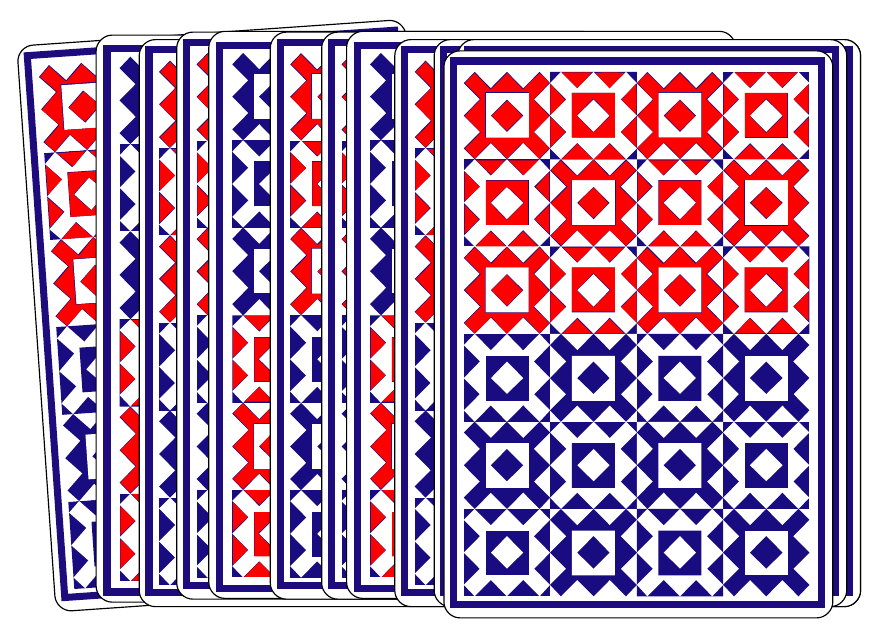
\includegraphics[scale=.7]{images/Trick2}
\caption{Flawed card backs allow the magician to see when a card is
  ``upside-down'' in the deck.}
\label{fig:trick2}
\end{figure}

The key to this trick lies in the magician's choice of deck.  Many cheaper card
decks, such as those given away as branded merchandise,
have corporate logos or
text on the card back that can 
provide information about how a card is oriented in the deck.  Because the trick
begins with a fresh deck, all cards are oriented in the same direction.  As a
result, when the volunteer is returning their card to the deck, the magician
simply has to orient the deck in such a way that the volunteer's card. is returned
in the opposite direction. During all shuffling
operations, the magician may maintain this orientation by rotating one pack of a
cut deck so that it's post-shuffle orientation matches the other pack.
To complete the trick, the magician only has to look through the deck of cards
and find the card with a differing orientation.  Figure~\ref{fig:trick2}
illustrates the magician's view of the deck of cards before the trick's
reveal.

%\subsubsection{Variations}
%
%...

\subsubsection{Lesson Takeaway}

Side channel attacks are not easily spotted.  Our goal is to
open the participant's eyes to the less
obvious avenues an attacker might use.
The reveal of this trick shows how we must not
take anything at face value, including what information
a card can contain.
Graphics on a card's back and even its orientation in a
deck enable the magician to identify a card. This is much like the way physical phenomena,
such as temperature, sound, and even electromagnetic output can
leak private data.
Thus, the trick provides a framework
to discuss side channels
as a security weakness that has nothing to do with a flaw in an
algorithm.
In order to emphasize the impact of such attacks we cover two examples: Van
Eck Phreaking and the SPECTRE vulnerabilities.
The former is a technique where images displayed by a computer monitor can be
detected and reconstructed using off-the-shelf radio hardware.
The latter is a major vulnerability recently discovered in many 
processors that use timing information to extract sensitive data from a
computer's memory.
The lesson concludes with tips on how to
reduce the risk of a side channel attack
by minimizing the number of potential channels,
and actively working to decouple potential
side channels from secret information.

\subsection{Attacks on Randomness}


True randomness is important in many
security-sensitive situations.
An attacker who is able to predict or influence the output of a random number
generator may use this capability to circumvent cryptographic security controls.
The trick we use to cover this concept
illustrates a potential vulnerability in cryptographic hash functions
-- that the last input to the function has a high degree of control over
the function's output.

Our trick relies on a foundational technique called ``forcing a card,''
defined as a ``a method of controlling a choice made by a spectator during
a trick~\cite{forcingcard}.''
In this case, the forcing relies on how the card in question is positioned
in the deck, how the deck is shuffled, and the magician's control over the
random number generator.

\subsubsection{From the Audience's Perspective}

The trick begins with the magician announcing that it is possible to
guess the value of any card randomly selected from a deck due to the different amounts of ink on its face.
This gives each card
a unique
weight that can be detected by feel.
To prove this point,
The magician spreads a deck of cards on the table face up
in order to prove its authenticity,
shuffles the deck,
and deals five cards out on the table.
The magician will make a prediction from these cards.
In order to head off suspicion that a specific card made it into the candidate set, the magician reveals that
a software random number generator will be used to select the card to be
guessed.
Students are asked to shout out numbers to be fed into the random number
generator to seed its operation.  After many numbers have been input, the
magician generates a number between 1 and 5, with each value referring to a
specific card.  The magician moves the chosen card forward and slides it back
and forth on the table to get an idea of its weight,  makes
a prediction, and reveals that it is correct!

\subsubsection{Behind the Scenes}

\begin{figure}[H]
\centering
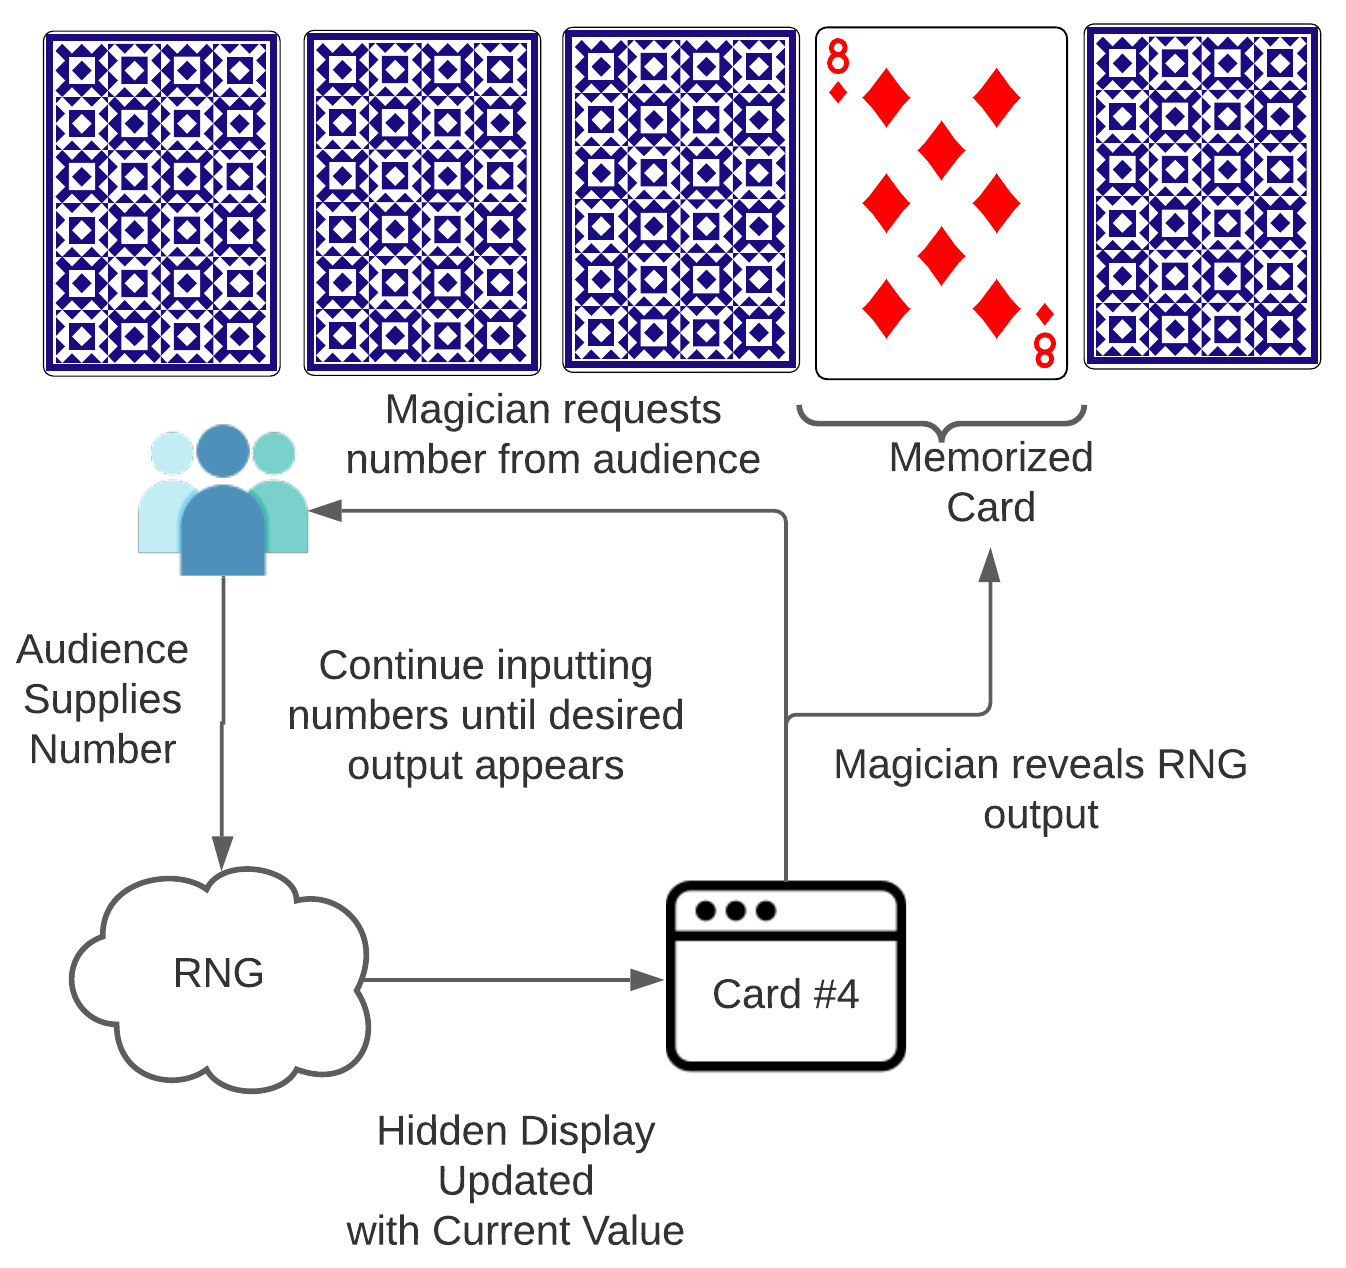
\includegraphics[scale=.6]{images/Trick3}
\caption{Participant are fed into our ``random number generator.''  The magician stops entering inputs
when a hidden display indicates a memorized card would be chosen.}
\label{fig:trick3}
\end{figure}

The success of this trick relies on two elements.
The first is when the deck is spread out on the
table before the students.  This movement serves the dual purpose of convincing
the students that the deck is genuine and gives the magician a chance to
memorize one or more of the top five cards in the deck.
When the deck is
shuffled, the magician is careful to not allow the cards that were memorized to
become mixed in with the rest of the deck.  This is easily accomplished by
using a standard riffle shuffle and ensuring that the top several cards of
the deck are allowed to fall as a unit after the remainder of the deck has
been shuffled normally~\cite{wikishuffle}.
Keeping the top of the deck intact allows them to ensure that
these cards will be dealt onto the table prior to making a prediction.


The second key lies in how the random number is generated.
Rather than
a true software random number generator, the magician's tool is based on a hash
function.  This means that, while output appears random, it is anything but.
As the students' shouted numbers are fed into the tool, the magician monitors an
intermediate output.
This output shows the result of first feeding a student's number
into the hash function. Modulus is used to reduce the output to a value
between zero and four. By adding one, you  get a value between
one and five.
The magician can use this input to determine when the output will be a number
corresponding with a card they have memorized and stop supplying inputs.
Figure~\ref{fig:trick3} illustrates how these two pieces interact to make
the trick work.


%\subsubsection{Variations}
%
%...

\subsubsection{Lesson Takeaway}

The purpose of this lesson is to show students the importance of correct
randomness
that is "fit for purpose," or appropriate for security-sensitive applications.
It also shows how an attacker
with a small amount of influence,
such as when to stop supplying numbers,
can compromise a
system.
As such, we begin by covering the common pitfalls
that occur when generating and
using randomness.
This foundation is used to explain both
direct and input-based attacks on random
number generators.
The explanation of these attacks gives our students the background they need to
understand why the magician's random number generator was invalid as well as
many of the most important properties of cryptographic hash functions.

%The trick we use reinforces this using
%a situation where ``users'' are able to provide input
%directly to a cryptographic hash function.
%We build on this by discussing how these functions work and their importance
%in applications like cryptocurrency and password storage.

%\section{Architecture}
\label{SEC:architecture}

[This is how the system actually works.  Go in depth with the design, but 
don't describe implementation details (most of the time).  That usually
goes in a separate impl section.  So, explain the commonalities if someone 
implement it on a different OS w/ a different language, using different
file formats, etc.]

[Diagrams are useful here.  This is usually 2-3 pages and can also have 
multiple sections]



%\section{Implementation (sometimes rolled into eval)}
\label{SEC:implementation}

Our reference implementation for XYZ is available with an MIT license at
XYZ. It utilizes ...  The source code is written in 4,324 lines of Python code
according to SLOCCOUNT (cite).


\section{Study Instrument and Evaluation}
\label{SEC:evaluation}

\subsection{Method}

The goal of our study was to judge how effective a non-traditional approach
could be in teaching novices about our selected attacks.  To do so,
we put together a 90 minute Zoom session to be presented at a summer
computer science workshop for high school students.  The session was
offered twice during the three week workshop, with the lead investigator
serving as the presenter and magician.  It was divided into three phases,
one
for each topic,
and each phase consisted of a performance of the topic's magic
trick, followed by a detailed discussion that used the magic trick
as a scaffold.  A total of 15 students attended the two sessions.

To measure improvements in participants' mastery of the subject, we
designed an assessment instrument (shown in figure~\ref{fig:assessment})
consisting of
12 multiple choice questions (4 for each topic),
3 Likert-scale survey statements,
and a free response comments section.
All of these materials were reviewed and approved by our university's
Institutional Review Board and, though attendance was open to all, we only
used data from students who had given us their consent to be part of the
study.

Participants completed the 12 multiple choice questions twice,
once before our lecture to gather a baseline of
participants' existing knowledge of the material,
and again at the conclusion of our
lecture as a post-test to determine if student mastery improved.
Both assessments used the same questions.
After taking part in the workshop, participants also evaluated the session
itself by offering opinions on whether or not they found our lecture
enjoyable and engaging.
The post-test was handed out at the conclusion of the lesson
and students were asked
to complete it in their own time.
Of the 15 students that attended our session, 10 agreed to participate in
the study and completed our pre-test. Of these 10, 5
students completed our post-test and survey.  Given the overwhelmingly
positive feedback we received from our session attendees, we believe the
decreased number of participants completing the post test can likely
be attributed
to the awkwardness of an interactive session online
rather than deficiencies in
the session itself.


\begin{figure*}[htb!]
  \scriptsize
  \begin{tabular}{c | p{8cm} | c | p{8cm}}
   & Question Text  &     & Question Text\\
\hline
Q1 & Which of the following is the best definition of social engineering  & Q2  & The act of creating a scenario in order to extract information is called:   \\
Q3 & What of the following pieces of information are dangerous to reveal online?  & Q4  & Bad actors can use stolen personal information to do which of the following: \\
Q5 & What is a side channel attack?  & Q6  & Which of the following can give you a hint as to what a computer is doing?   \\
Q7 & What is an example of a common real-world side channel attack?  & Q8  & How could you prevent an attacker from stealing a password by using a microphone to listen to keystrokes?\\
Q9 & Which of the following is a major use of hash functions? & Q10 & Which of the following is an important feature of a good hash function  \\
Q11 & When passing multiple items sequentially into a hash function, which item has the most influence on the output & Q12 & What is the term used when two or more inputs to a hash function generate the same output? \\
\hline
S1 & The lesson today increase my knowledge in the areas we covered. & S2  & The manner in which the material was presented helped me understand the material better\\
S3 & I enjoyed the manner in which the material was presented &     &              \\
\end{tabular}
\caption{Questions used in our study instrument.  Questions Q1 through Q12
    appeared on both the pre-test and post-test.  Statements S1 through S3
    appeared only on the post-test.}
\label{fig:assessment}
\end{figure*}


\subsection{Results}

\begin{figure}
  \centering
\subfloat[Aggregate results showing number of correct responses and percent of correct responses for each question on both our pre-test and post-test.  Percent correct is based on our total of five responses.]{
  \begin{tabular}{c | l | l | l}
Question &  Correct on Pre-test   & Correct on Post-test \\
\hline
Q1   & 3 (60\%)  & 5 (100\%) \\
Q2   & 3 (60\%)  & 4 (80\%)  \\
Q3   & 5 (100\%) & 5 (100\%) \\
Q4   & 2 (40\%)  & 5 (100\%) \\
Q5   & 0 (0\%)   & 0 (0\%)   \\
Q6   & 5 (100\%) & 5 (100\%) \\
Q7   & 4 (80\%)  & 5 (100\%) \\
Q8   & 3 (60\%)  & 5 (100\%) \\
Q9   & 4 (80\%)  & 3 (60\%)  \\
Q10  & 4 (80\%)  & 4 (80\%)  \\
Q11  & 1 (20\%)  & 5 (100\%) \\
Q12  & 2 (40\%)  & 5 (100\%) \\
  \end{tabular}}

\subfloat[Rows S1, S2, and S3 report number of participants that selected the listed response.  Likert responses that were not chosen by any participant are omitted.]{
\begin{tabular}{ c | l}
Statement & Aggregate Responses \\
\hline
S1 &  Strongly Agree: 4 Agree: 1 \\
S2 &  Strongly Agree: 4 Agree: 1 \\
S3 &  Strongly Agree: 5 \\
\end{tabular}}
\caption{Results from our pre-test, post-test, and survey}
\label{fig:results}
\end{figure}

Overall, aggregate scores, shown in Figure~\ref{fig:results},
increased across all categories on the post-test.
Scores for the social engineering and attacks on randomness sections
increased by 30\% while the side channel attacks section increased by
15\%.

The improvement in social engineering scores can be traced to
higher scores on
Q1, Q2, and Q4.
This indicates a better understanding of the technical details
around social engineering.
Encouragingly, the students were well aware of
what information should not be shared online suggesting they have been
warned about these dangers in other places.

The improvements in scores related to attacks on randomness
came largely
from more accurate responses to Q11 and Q12.
These questions are particularly important because
correct answers suggest the students have learned two
key properties of hash functions.
The fact Q9 scores improved a small amount and Q10 scores did not improve
means future iterations of the lesson should spend more time
explaining how these functions may be used in the real world.

The smallest improvement (15\%) came about in the side channel attacks
scores.  This is largely due to Q9 which proved difficult for students on
both the pre-test and post-test.  We believe this indicates a flaw in this
question and it will be reworked for future sessions.

In terms of student opinions about the lessons, Figure~\ref{fig:results}
shows the session scored very highly
on our Likert-scale statements.  A significant majority of students strongly
agreed that the lesson improved their skills in the covered topics.  A
similar majority felt the magic-based presentation was useful and
enjoyable.  A few students offered free response comments describing the
session as ``fun,'' ``entertaining,'' and ``interesting.''  One response
stated that the side-channel attack using upside-down cards
was particularly useful for helping them understand how such attacks are
structured.


%Comparing aggregate pre-test and post-test results show an improvement of
%AAA\%.  The majority of this improvement came from better scores on the
%hash function-related questions.  This improvement likely comes from our
%participant population's lack of experience with the area.  The details of
%hash functions are likely to be covered in undergraduate course work rather
%than high-school computer science classes.
%
%The next most-improved topic was side channel attacks.  Questions 6 and 7
%showed a marked improvement from AAA\% correct to BBB\% correct.  Answering
%these questions correctly requires students to understand the theory
%behind side
%channel attacks and apply it to several scenarios to identify the correct
%response.  As a result,  improved scores on these questions indicate deeper
%mastery of the material rather than simple memorization of a definition.
%
%The questions related to social engineering showed some improvement, though less
%than the other areas.  This is due to most participants correctly answering
%these questions on the pre-test.  It is likely students currently
%attending high school grew up in a time where education about scams and
%safety on the internet has been ongoing from an early age.


\subsection{Instructor Observations}

Based on instructor observation, student experience during
each session was overwhelmingly positive --
particularly in light of the teaching modality enforced by COVID-19
restrictions.
Of particular importance are two key indicators
of student engagement in a remote setting: camera usage and
responsiveness.  In both sessions a high majority of students used their
cameras when participating in a trick, asking, and answering questions
about the material.  Students remained attentive and focused throughout
 the lesson suggesting that our
style of presentation can help maintain attention during a moderately long,
technical lecture.

Student responsiveness during both sessions was very high.
They were eager to analyze the
tricks and put forward hypotheses about how they worked.
When prompted to
expand on certain aspects of the material, students quickly volunteered and
offered responses indicating a growing understanding of the topic.
Further, students readily volunteered to participate in the tricks in spite
of the unusual teaching modality created by a remote presentation,
along with the general discomfort of being in a
prominent position ``at the front of class.''

After the session,
unprompted verbal comments attest to the lesson's effectiveness.
Students volunteered that they enjoyed the
lesson and found the magic tricks aided their understanding of the
material.  These comments support the appeal of our lesson's approach and
encourage its use in this and other subject areas.

\section{Related Work}
\label{SEC:related-work}

The idea of scaffolding is to provide a bridge to assist students
in mastering material that may be beyond their reach~\cite{wood1976role}
by bringing it into what psychologist Lev Vygotsky described as a student's
``Zone of Proximal Development.~\cite{vygotsky1978}''  Given the complexity of computer science
topics, it is not surprising that researchers have attempted to ``scaffold''
these concepts from a familiar base.  In a meta-analysis from 2019, Szabo et al.
identified 1283 papers in the field that contain scaffolding related
content~\cite{szabometa}.
Vanderyde et al. argues for greater use of scaffolding and engaging teaching
practices in order to improve learning in light of increased computer science
enrollment and diversity in computer science
Programs~\cite{vanderhydescaffolding}.  Stanier discusses
further success in using scaffolds to introduce new topics in a higher education
environment~\cite{stanierhighered}.
We believe the results show that our demonstrations work as
effective scaffolds for introducing novel security concepts to novices.

Other researchers have already integrated card tricks into lesson plans about
computer science concepts, such as using parity bits to detect unintended bit
flips, a central technique in error detection and correction.  Bell et al. uses a
5 by 5 grid of cards in an exercise that transforms the concepts into a hands-on
exercise~\cite{bell2009computer, csunplugged}.
The exercise improves students' understanding by allowing them to
both generate parity errors and participate in their detection.  Greenberg et
al. was able to create more advanced versions using larger grids.  Other versions
of this activity rely on software assistance to handle more complex
computations~\cite{Greenberg2017, Greenberg2018}.

In Ferreria et al. a ``self-working'' card trick called ``Are You Psychic?''
is used
as a medium to explain topics in algorithm analysis and design, such as problem
decomposition, pre- and post- conditions, and
invariants~\cite{ferreira2014magic}.
The trick's relevance
to each lesson is illustrated by mapping each of its steps onto a formal
description of the algorithm.  Garcia et al. have produced three papers describing
a wide variety of magic tricks, along with the computer science concepts they
can help teach~\cite{garcia2012demystifying,
garcia2013demystifying,
garcia2016demystifying}.
Their goal was to help students construct a mental model of how
a computer actually works, which they argue is an essential component of any
introductory course.  Similarly, Curzon et al. found success explaining computer
science concepts to younger students using magic shows~\cite{curzon2008engaging}.


%The card tricks and lessons we developed were inspired by previous research
%showing the effectiveness of magic to convey or explain computer science
%concepts.
%%We summarize these earlier initiatives in
%%Section~\ref{sec:magicineducation}, followed by a look at how card
%%demonstrations work as scaffolding devices in
%%Section~\ref{sec:demosasscaffolding}.
%
%\paragraph{Card Magic in Computing Education:}
%Given the complexity of many computer science topics, it's perhaps not
%surprising that the use of card magic to explain key concepts is already an
%established practice.  Below are a few examples from which we took inspiration
%when creating our information security-focused lessons.
%
%\paragraph{Error Correction and Parity}
%While using parity bits to detect unintended bit flips is a central technique
%in error detection and correction, it can sometimes seem unusual or unintuitive
%to novice computer scientists.
%The ``Computer Science Unplugged'' umbrella of teaching resources offers
%several examples.  Bell et al. uses
%a 5 by 5 grid of cards in an exercise designed to teach about parity and
%error correction by transforming the concepts into a hands on
%exercise~\cite{bell2009computer}~\cite{csunplugged}.  The exercise improves
%student's understanding by allowing them to both generate parity errors and
%participate in their detection.
%Greenberg et al. expand upon this style of trick by creating more advanced
%versions using larger grids.  Some new versions also use
%more complex error detection
%strategies to increase the size of the grid that can be handled by a human
%magician.  Others rely on software assistance to handle more complex
%computation~\cite{Greenberg2017}~\cite{Greenberg2018}.
%
%\paragraph{Algorithm Analysis and Design}
%Ferreira et al. use a ``self-working'' card trick called ``Are You Psychic''
%as a medium to explain topics
%like problem decomposition, pre- and post- conditions, and
%invariants~\cite{ferreira2014magic}.
%The trick's relevance to each lesson is illustrated by
%mapping each of its steps
%onto a formal description of the trick's algorithm.
%
%\paragraph{Multi-trick Magic Shows}
%Garcia et al. have produced three papers describing a wide variety of magic
%tricks, along with the computer sciences concepts they can help
%teach~\cite{garcia2012demystifying}
%~\cite{garcia2013demystifying}
%~\cite{garcia2016demystifying}.
%Their goal was to help students construct a mental model of how a computer
%actually works, which they argue is an essential component of any introductory
%course.
%Similarly, Curzon et al. found success explaining computer
%science concepts to younger students using magic shows~\cite{Curzon2008}.
%
%\paragraph{Demonstrations as Scaffolding}
%Our use of card tricks as scaffolding when introducing new concepts is also well
%supported by education literature.
%
%\paragraph{Why Magic Tricks work as Scaffolding}
%The purpose of our magic tricks and demonstrations is to introduce
%information security concepts in such a way that students from varying
%backgrounds are able to understand them.  This methodology has a long history of
%support, starting with psychologist Lev Vygotsky
%who described the need to bring topics into a
%student's ``Zone of Proximal Development.~\cite{vygotsky1978}''
%A common approach to performing this migration is to provide assistance in the
%form of ``scaffolding'' that can assist students in mastering material that may
%be beyond their reach~\cite{wood1976role}.  We believe our results show that our
%demonstrations are effective scaffolds for introducing novel security concepts
%to our participants.  Scaffolding is widely used in other areas and is something
%the information security community should consider employing to a larger degree.
%
%\paragraph{Use of Scaffolds in Computer Science Education}
%Perhaps because its core concepts can appear daunting to new students,
%the use of scaffolds in Computer Science education is well supported. In a
%meta-analysis from 2019 Szabo et
%al. identify 1283 papers in the field that contain scaffolding related
%content~\cite{szabometa}.
%Vanderyde et al. argues for greater use of scaffolding and
%engaging teaching practices in order to improve learning in light of increased
%Computer Science enrollment and diversity in Computer Science
%programs~\cite{vanderhydescaffolding}.  Stanier discusses further success in
%using scaffolds to introduce new topics in a higher education
%environment~\cite{stanierhighered}.

\section{Conclusion}
\label{SEC:conclusion}

On of the most difficult parts of planning an introductory information security
class is addressing the wide degree of backgrounds and aptitudes in a diverse
student body.
In this work we have presented a lesson plan for using card magic to each
information security concepts to novices.  Our use of this lesson plan in a
real-world teaching environment has shown that it is highly effective at both
fostering student engagement and improving their mastery of the covered
material.
We encourage our fellow educators to use the tricks we have developed and to
develop new tricks as a way to make complex and potentially intimidating
material more approachable for novice students with varying backgrounds.



{\footnotesize \bibliographystyle{abbrv}
\bibliography{bibdata}}

\end{document}
